\documentclass[11pt,conference]{IEEEtran}

\usepackage{cite}
\usepackage{amsmath,amssymb,amsfonts}
\usepackage{algorithmic}
\usepackage{graphicx}
\usepackage{textcomp}
\usepackage{xcolor}
\usepackage{booktabs}
\usepackage{longtable}
\usepackage{array}
\usepackage{multirow}
\usepackage{wrapfig}
\usepackage{float}
\usepackage{colortbl}
\usepackage{pdflscape}
\usepackage{tabu}
\usepackage{threeparttable}
\usepackage{threeparttablex}
\usepackage[normalem]{ulem}
\usepackage{makecell}

\def\BibTeX{{\rm B\kern-.05em{\sc i\kern-.025em b}\kern-.08em
    T\kern-.1667em\lower.7ex\hbox{E}\kern-.125emX}}

\begin{document}

\title{Analysis of Potential Connectomic Biomarkers for ASD using Machine Learning}

\author{
    \IEEEauthorblockN{Tony Kabilan Okeke}
    \IEEEauthorblockA{\textit{School of Biomedical Engineering} \\
    \textit{Drexel University}\\
    Philadelphia, PA \\
    tko35@drexel.edu}
}

\maketitle

\begin{abstract}
    In recent years, several studies have been conducted to investigate the structural and 
    functional alterations to the brain that are associated with various neurological 
    disorders and diseases. Great interest has been placed on the identification of 
    connectomic biomarkers for these disorders. With the aid of various machine learning 
    models -- including support vector machines and lasso regression -- this study aims 
    to identify potential structural biomarkers for ASD in children by analyzing a 
    collection of graph theory measures computed for connectomes of autistic and typically 
    developing children. The results of this study indicate that the distribution of 
    neuronal connections -- whether localized within subnetworks, or distributed across 
    the entire connectome -- could be a potential biomarker for ASD.
\end{abstract}

% ----------------------------------------------------------------------------------------

\section{Introduction}

Autism Spectrum Disorder (ASD) is a neurodevelopmental disorder that is characterized by 
social and communication deficits as well as restricted, repetitive behaviors. Early 
diagnosis and intervention are critical for improving long-term outcomes; however, the 
current gold standard assessment tools are limited in their ability to accurately and 
efficiently diagnose ASD, particularly in young children. Typically, ASD diagnoses are 
based on behavioral criteria, but there is growing interest in the identification of 
objective biomarkers to aid in the diagnoses \cite{Shen.2019}. Biomarkers are measurable 
characteristics that can be used to indicate the presence or severity of a disease. In the 
case of ASD, biomarkers could be used to improve and validate diagnoses, especially in 
young children, and potentially before the emergence of symptoms.

Due to advancements in multimodal neuroimaging in recent years, neuroscience has gained 
unprecedented opportunities to interrogate the living human brain at multiple scales in 
both health and disease \cite{Hong.2019}, and these advancements have been especially 
useful in the study of neurodevelopmental disorders \cite{Nunes.2019}. The field of 
network neuroscience aims to investigate such disorders by leveraging magnetic resonance 
imaging (MRI) and and various tractography algorithms to construct `brain graphs' or 
`connectomes' which are matrix representations of the structural and/or functional 
connections between various regions of the brain; these connectomes serve as useful tools 
for the analysis of neurological disorders and diseases by providing insight into how 
the connections within the brain are altered in such diseases or disorders.

Several studies have been conducted to examine changes in functional connectivity in 
individuals with ASD relative to typically developing controls \cite{Lau.2019, Williams.2013}. 
However, less is known about changes in structural connectivity in individuals with ASD. 
Recent studies have investigated the differences between the brains of patients with ASD 
and typically developing controls by comparing graph theory measures computed on their
connectomes \cite{Roine.2015}. By capitalizing on diffusion-weighted magnetic resonance 
imaging (dMRI), previous studies were also able to identify abnormalities in the connectivity 
strength of several inter-regional fiber pathways in individuals with ASD \cite{dAlBbis.2018}. 
Despite the identification of these abnormalities, the diagnosis of ASD based on brain 
imaging remains a challenge. One reason for this challenge is that the abnormalities 
associated with ASD are often subtle and are often difficult to detect. This calls for the 
application of sophisticated computational methods to aid in the diagnoses.

In recent years, the application of machine learning tools has become a major part of 
network neuroscience \cite{Abos.2017,Vogt.2018}. Some researchers studying ASD have 
developed classifiers - machine learning models that predict whether a connectome is from 
a subject with ASD or not - for identifying ASD connectomes. One such study involved the 
development of convolutional neural network architecture for the prediction of cognitive 
and motor scores from the connectomes of infants born preterm \cite{Kawahara.2017}.
Another study showed that the functional connectome of a subject at six months old could 
be used to accurately predict whether or not the subject would have developed ASD by 
their second birthday using machine learning models including neural networks,
support vector machines, and random forests \cite{Horien.2022}.

The goal of this study is utilize a combination of machine learning models to identify and 
evaluate the diagnostic accuracy of potential connectomic biomarkers for ASD. Additionally, 
I will analyze the relationships between the potential connectomic biomarkers and autism 
severity, social communication and intelligence as assessed by the Autism Diagnostic 
Observation Schedule Clinical Severity Score (ADOS-CSS), Social Communication 
Questionnaire (SCQ), and Intelligence Quotient (IQ) respectively.

% ----------------------------------------------------------------------------------------

\section{Methods}

\begin{figure}[ht]
    \vskip 0.2in
    \begin{center}
        \centerline{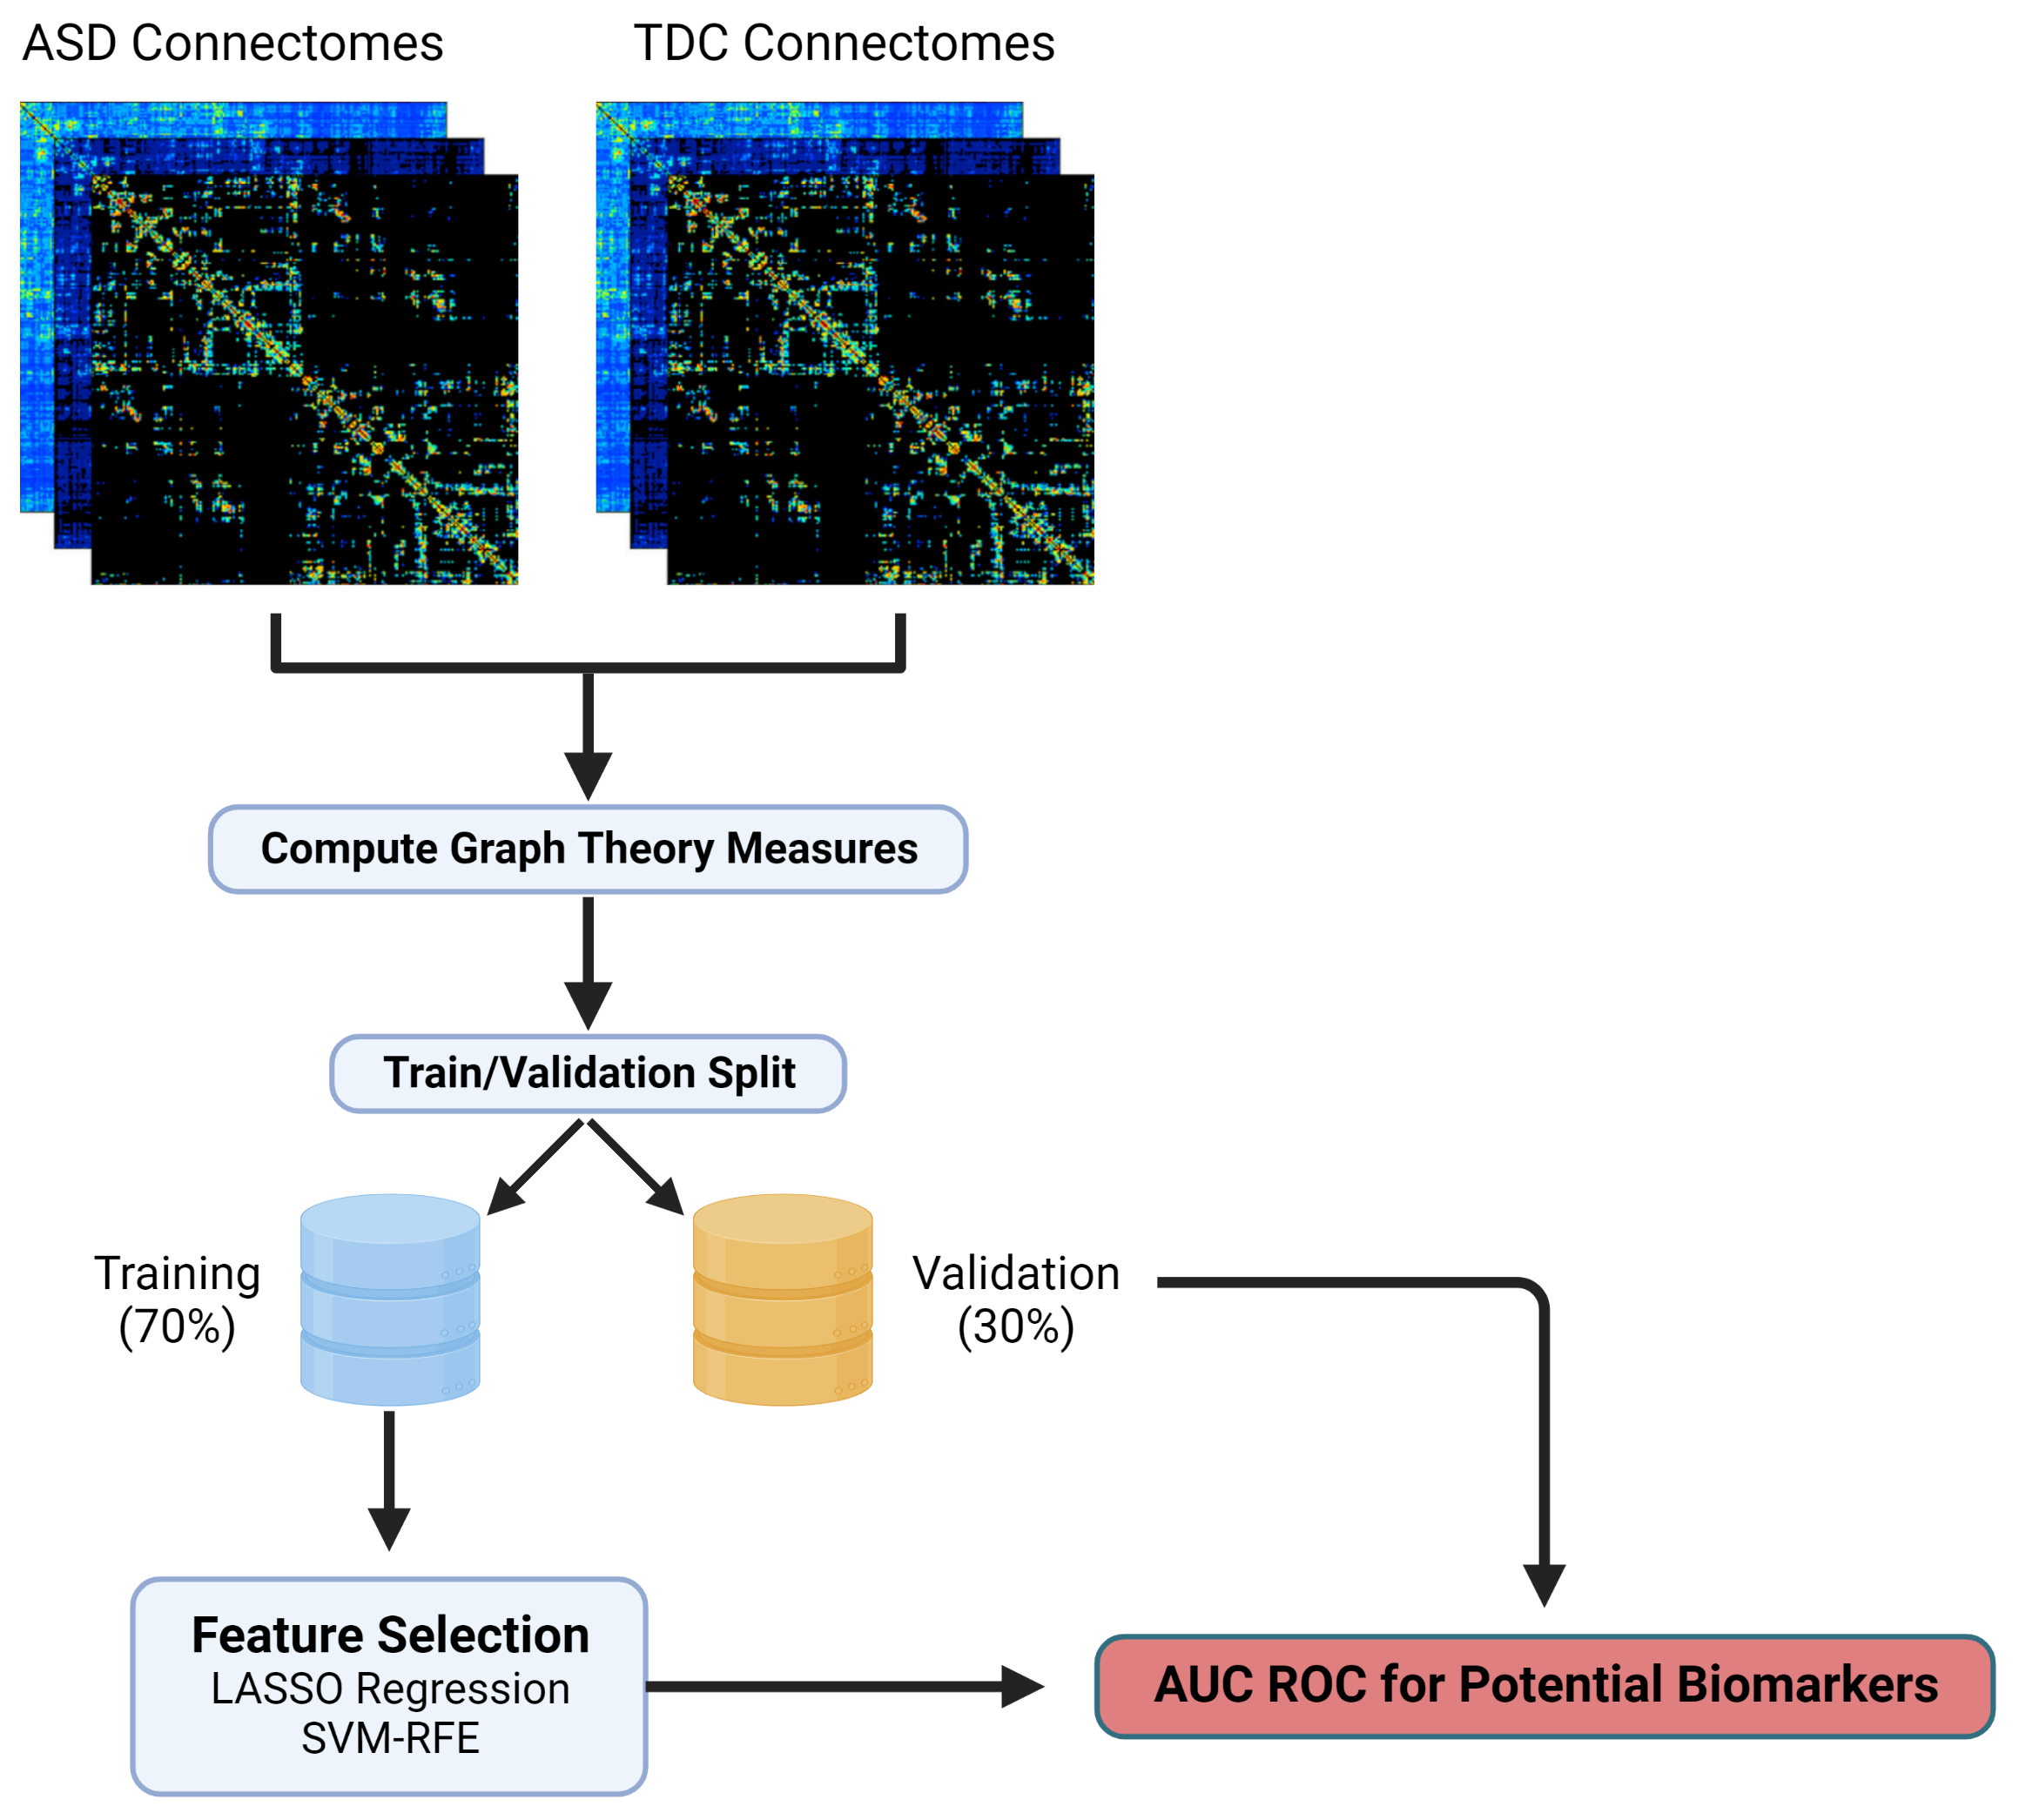
\includegraphics[width=\columnwidth]{../img/project_schematic_final.png}}
        \caption{
            Overview of autism biomarker identification using machine learning models.
            Graph theory measures are computed for both ASD and TDC connectomes, the 
            data is split for training and validation. Training data is used to perform 
            feature selection using LASSO regression and SVM-RFE based selection. The 
            selected features are then used to evaluate the AUC ROC using the validation 
            dataset.
        }
        \label{project-schematic}
    \end{center}
    \vskip -0.2in
\end{figure}

\subsection*{\textbf{Dataset}}
    The data analysis workflow for this study is shown in Fig. \ref{project-schematic}.
    This study was performed on the CHARM dataset provided by collaborators at Penn 
    Medicine. dMRI scans were collected from a cohort of 450 children between 6 and 19 
    years old across 11 different sites. Of the 450 subjects involved, only 313 were 
    included in the final dataset following data quality assessment. The study cohort 
    included 163 children with ASD ($\text{age}=12.10~\pm~2.76$; 133 males; 30 females) 
    as well as 150 typically developing controls (TDCs) ($\text{age}=11.87~\pm~2.82$; 
    115 males; 35 females). For each subject, only a single dMRI scan was performed. 
    The age, sex, SCQ and IQ scores were recorded for all subjects in the cohort. The 
    SCQ score is considered the gold-standard measure for assessing communication skills
    and ranges from 0 to 39; a score of 15 or higher is considered indicative of ASD, 
    whereas a score of 14 or below is within the range of typical development. For 
    subjects with ASD, the ADOS-CSS was also recorded. The ADOS-CSS is a semi-structured, 
    play-based assessment administered by a trained professional; it is the gold-standard 
    measure for assessing autism severity and ranges from 1 to 10, with higher scores
    indicating greater autism severity.

\subsection*{\textbf{Connectomes}}
    Two structural connectomes were constructed from the dMRI image of each subject in the 
    cohort. The first set of connectomes were constructed using the Desikan atlas with
    86 parcellations, while the second set of connectomes were constructed using the 
    Schaefer atlas with 220 parcellations. The adjacency matrices for the connectomes were 
    stored in tab-delimited text files. The adjacency matrices for the Desikan connectomes 
    are 86 x 86 in size, while those for the Schaefer connectomes are 220 x 220 in size.
    The edge weights for both sets of connectomes were computed using tractographic tools.
    The diagonal entries in the connectomes were set to 0 to exclude any self connections 
    that may exist within the data. Both sets of connectomes were analyzed using the 
    workflow described in Fig. \ref{project-schematic}.

\subsection*{\textbf{Comparison of Graph Theory Measures}}
    The `bctpy' package -- a python-based implementation of the Brain Connectivity 
    Toolbox (BCT) -- was used to compute graph theory measures \cite{Rubinov.2010.BCT}.
    A total of 22 network-level graph theory measures were computed for each connectome; 
    these measures were selected because they have been previously identified as being
    distinctive in ASD connectomes \cite{Roine.2015,Craddock.2013}.
    The group differences between ASD and TDC connectomes were computed for each measure 
    using the student's t-test, along with Cohen's D effect sizes and p-values; the 
    p-values were corrected for multiple comparisons using the \textit{Benjamini-Hochberg} 
    method. Measures with corresponding p-values less than 0.05 were considered significant 
    and used as candidate biomarkers for feature selection. The corresponding node-level 
    measures for the candidate biomarkers were also computed and used as addition features 
    for the machine learning models used for the identification of potential biomarkers.

\subsection*{\textbf{Identification of Potential Biomarkers}}
    Multiple feature selection techniques were utilized for the identification of 
    potential biomarkers from the candidates. This analysis was conducted in `python' 
    using the `scikit-learn' package \cite{sklearn}. A combination of the significantly 
    different network-level graph theory measures and their corresponding node-level 
    measures were used for feature selection.

    The dataset was split into a training set (70\%) and a validation set (30\%). The 
    training set was used to train the LASSO regression and SVM models and to perform 
    feature selection. The validation set was used to construct ROC curves to evaluate 
    the accuracy of the biomarkers.

    LASSO regression is a machine learning algorithm that is typically used to improve 
    the prediction accuracy of some other model by selecting a subset of features.
    LASSO regression is widely used for feature selection and has been used to screen out 
    diagnostic or prognostic factors from genomic datasets \cite{Wang.2019}. One recent 
    study used LASSO regression to identify sub-type specific biomarkers for breast 
    cancer survivability \cite{Jubair.2020}. We utilized LASSO regression to identify the 
    first set of potential biomarkers. When the model is trained, it attempts to minimize 
    its' cost function by selecting features that are useful in predicting the target 
    variable and discarding any redundant features. We performed a grid search with 5-fold 
    cross validation to find the optimal value of the regularization parameter, $\alpha$. 
    We then selected any features with non-zero coefficients in the model.

    To identify the second set of potential biomarkers, we utilized the Support Vector 
    Machine (SVM) algorithm with a linear kernel. SVM is widely used for solving both 
    classification and regression problems, and is often paired with Recursive Feature 
    Elimination (RFE) in biomarker discovery studies. The model has nonlinear discrimination 
    characteristics which allow results to be compared across models trained with different 
    numbers of features to identify the optimal combination of features. One recent study 
    used SVM to screen out 10 discriminant features which provide a fast and effective 
    diagnostic standard for Kashin-Beck disease \cite{Zhang.2021}. We performed a grid 
    search to optimize the hyperparameters of the Linear Support Vector Classifier 
    (LinearSVC) and utilized RFE to identify the second set of potential biomarkers.

\subsection*{\textbf{Diagnostic Accuracy of Potential Biomarkers}}
    Receiver Operating Characteristic (ROC) curves were generated for each of the 
    potential biomarkers. Each set of potential biomarkers was used to construct a 
    LinearSVC to distinguish between ASD and TDC connectomes. The area under the 
    curves (AUCs) were used to determine the diagnostic accuracy of each potential 
    biomarker.

\subsection*{\textbf{Correlation with Clinical Outcomes}}
    To further assess the relationship between the potential biomarkers and autism 
    severity, the correlation coefficients between each biomarker and the ADOS-CSS, SCQ 
    and IQ scores were computed. The results were visualized using the `ggplot2` and
    `ggpubr' packages in `R' \cite{ggplot2,R-Core}.

% ----------------------------------------------------------------------------------------

\section{Results}

\subsection*{\textbf{Comparison of Graph Theory Measures}}

    The results of the group difference analyses are shown in Tables 
    \ref{group-diff-desikan} and \ref{group-diff-schaefer} (for Desikan and Schaefer 
    connectomes respectively). The p-values were corrected using the 
    \textit{Benjamini-Hochberg} method, and cohen's D effect sizes were computed.
    
    For the Desikan connectomes, `Average Degree', `Average Degree between Module', 
    `Average Interhemispheric Degree', `Average Degree within Module', `Density', and 
    `Average Eigenvector Centrality' were found to have significant (unadjusted) p-values. 
    Only `Average Degree within Module' was significant after p-value correction with an \
    effect size of -0.489. For the Schaefer connectomes, no measures were found to be 
    significant. Fig. \ref{group-diff-boxplots} shows boxplots comparing 
    the six significantly different measures.

    \begin{table}
        \caption{Group Differences between ASD and TDC for Network-Level Graph Theory
                    Measures of Desikan Connectomes}
        \begin{center}
            \begin{tabular}{p{4cm}p{1cm}p{1cm}p{1cm}}
                \toprule
                                                Measure &  P Value &  Adjusted P Value &  Effect Size \\
                \midrule
                                            Assortativity &    0.154 &             0.443 &       -0.161 \\
                            Characteristic Path Length &    0.602 &             0.761 &       -0.059 \\
                        Average Clustering Coefficient &    0.375 &             0.761 &        0.101 \\
                                \textbf{Average Degree} &    0.011 &             0.060 &       -0.289 \\
                \textbf{Average Degree between Module} &    0.018 &             0.084 &       -0.267 \\
                \textbf{Average Interhemispheric Degree} &    0.005 &             0.060 &       -0.315 \\
                        Average Intrahemispheric Degree &    0.497 &             0.761 &       -0.076 \\
                    \textbf{Average Degree within Module} &    0.000 &             0.000 &       -0.489 \\
                                        \textbf{Density} &    0.011 &             0.060 &       -0.289 \\
                                                Diameter &    0.735 &             0.768 &       -0.038 \\
                                    Average Eccentricity &    0.614 &             0.761 &       -0.057 \\
                 \textbf{Average Eigenvector Centrality} &    0.050 &             0.191 &        0.223 \\
                                        Global Efficiency &    0.531 &             0.761 &        0.071 \\
                                        Global Modularity &    0.090 &             0.295 &        0.192 \\
                    Average Node Betweenness Centrality &    0.367 &             0.761 &        0.102 \\
                        Average Participation Coefficient &    0.958 &             0.958 &       -0.006 \\
                                                Radius &    0.671 &             0.761 &       -0.048 \\
                                        Global strength &    0.629 &             0.761 &        0.055 \\
                            Global Off-Diagonal strength &    0.600 &             0.761 &        0.059 \\
                        Global Interhemispheric Strength &    0.421 &             0.761 &       -0.091 \\
                        Global Intrahemispheric Strength &    0.508 &             0.761 &        0.075 \\
                        Global Self Connections Strength &    0.695 &             0.761 &        0.044 \\
                \bottomrule
            \end{tabular} 
            \label{group-diff-desikan}
        \end{center}
    \end{table}
    
    \begin{table}
        \caption{Group Differences between ASD and TDC for Network-Level Graph Theory
                    Measures of Schaefer Connectomes}
        \begin{center}
            \begin{tabular}{p{4cm}p{1cm}p{1cm}p{1cm}}
                \toprule
                                            Measure &  P Value &  Adjusted P Value &  Effect Size \\
                \midrule
                                        Assortativity &    0.818 &             0.995 &       -0.026 \\
                            Characteristic Path Length &    0.871 &             0.995 &       -0.018 \\
                        Average Clustering Coefficient &    0.732 &             0.995 &        0.039 \\
                                        Average Degree &    0.721 &             0.995 &       -0.041 \\
                        Average Degree between Module &    0.700 &             0.995 &       -0.044 \\
                    Average Interhemispheric Degree &    0.688 &             0.995 &       -0.046 \\
                    Average Intrahemispheric Degree &    0.948 &             0.995 &       -0.007 \\
                        Average Degree within Module &    0.947 &             0.995 &        0.007 \\
                                            Density &    0.721 &             0.995 &       -0.041 \\
                                            Diameter &    0.841 &             0.995 &       -0.023 \\
                                Average Eccentricity &    0.991 &             0.995 &       -0.001 \\
                        Average Eigenvector Centrality &    0.647 &             0.995 &       -0.052 \\
                                    Global Efficiency &    0.956 &             0.995 &        0.006 \\
                                    Global Modularity &    0.995 &             0.995 &        0.001 \\
                Average Node Betweenness Centrality &    0.831 &             0.995 &       -0.024 \\
                    Average Participation Coefficient &    0.289 &             0.995 &        0.120 \\
                                                Radius &    0.823 &             0.995 &       -0.025 \\
                                    Global strength &    0.901 &             0.995 &        0.014 \\
                        Global Off-Diagonal strength &    0.967 &             0.995 &       -0.005 \\
                    Global Interhemispheric Strength &    0.692 &             0.995 &       -0.045 \\
                    Global Intrahemispheric Strength &    0.989 &             0.995 &        0.002 \\
                    Global Self Connections Strength &    0.842 &             0.995 &        0.023 \\
                \bottomrule
            \end{tabular}                                                      
            \label{group-diff-schaefer}
        \end{center}
    \end{table}

    \begin{figure}
        \vskip 0.2in
        \begin{center}
            \centerline{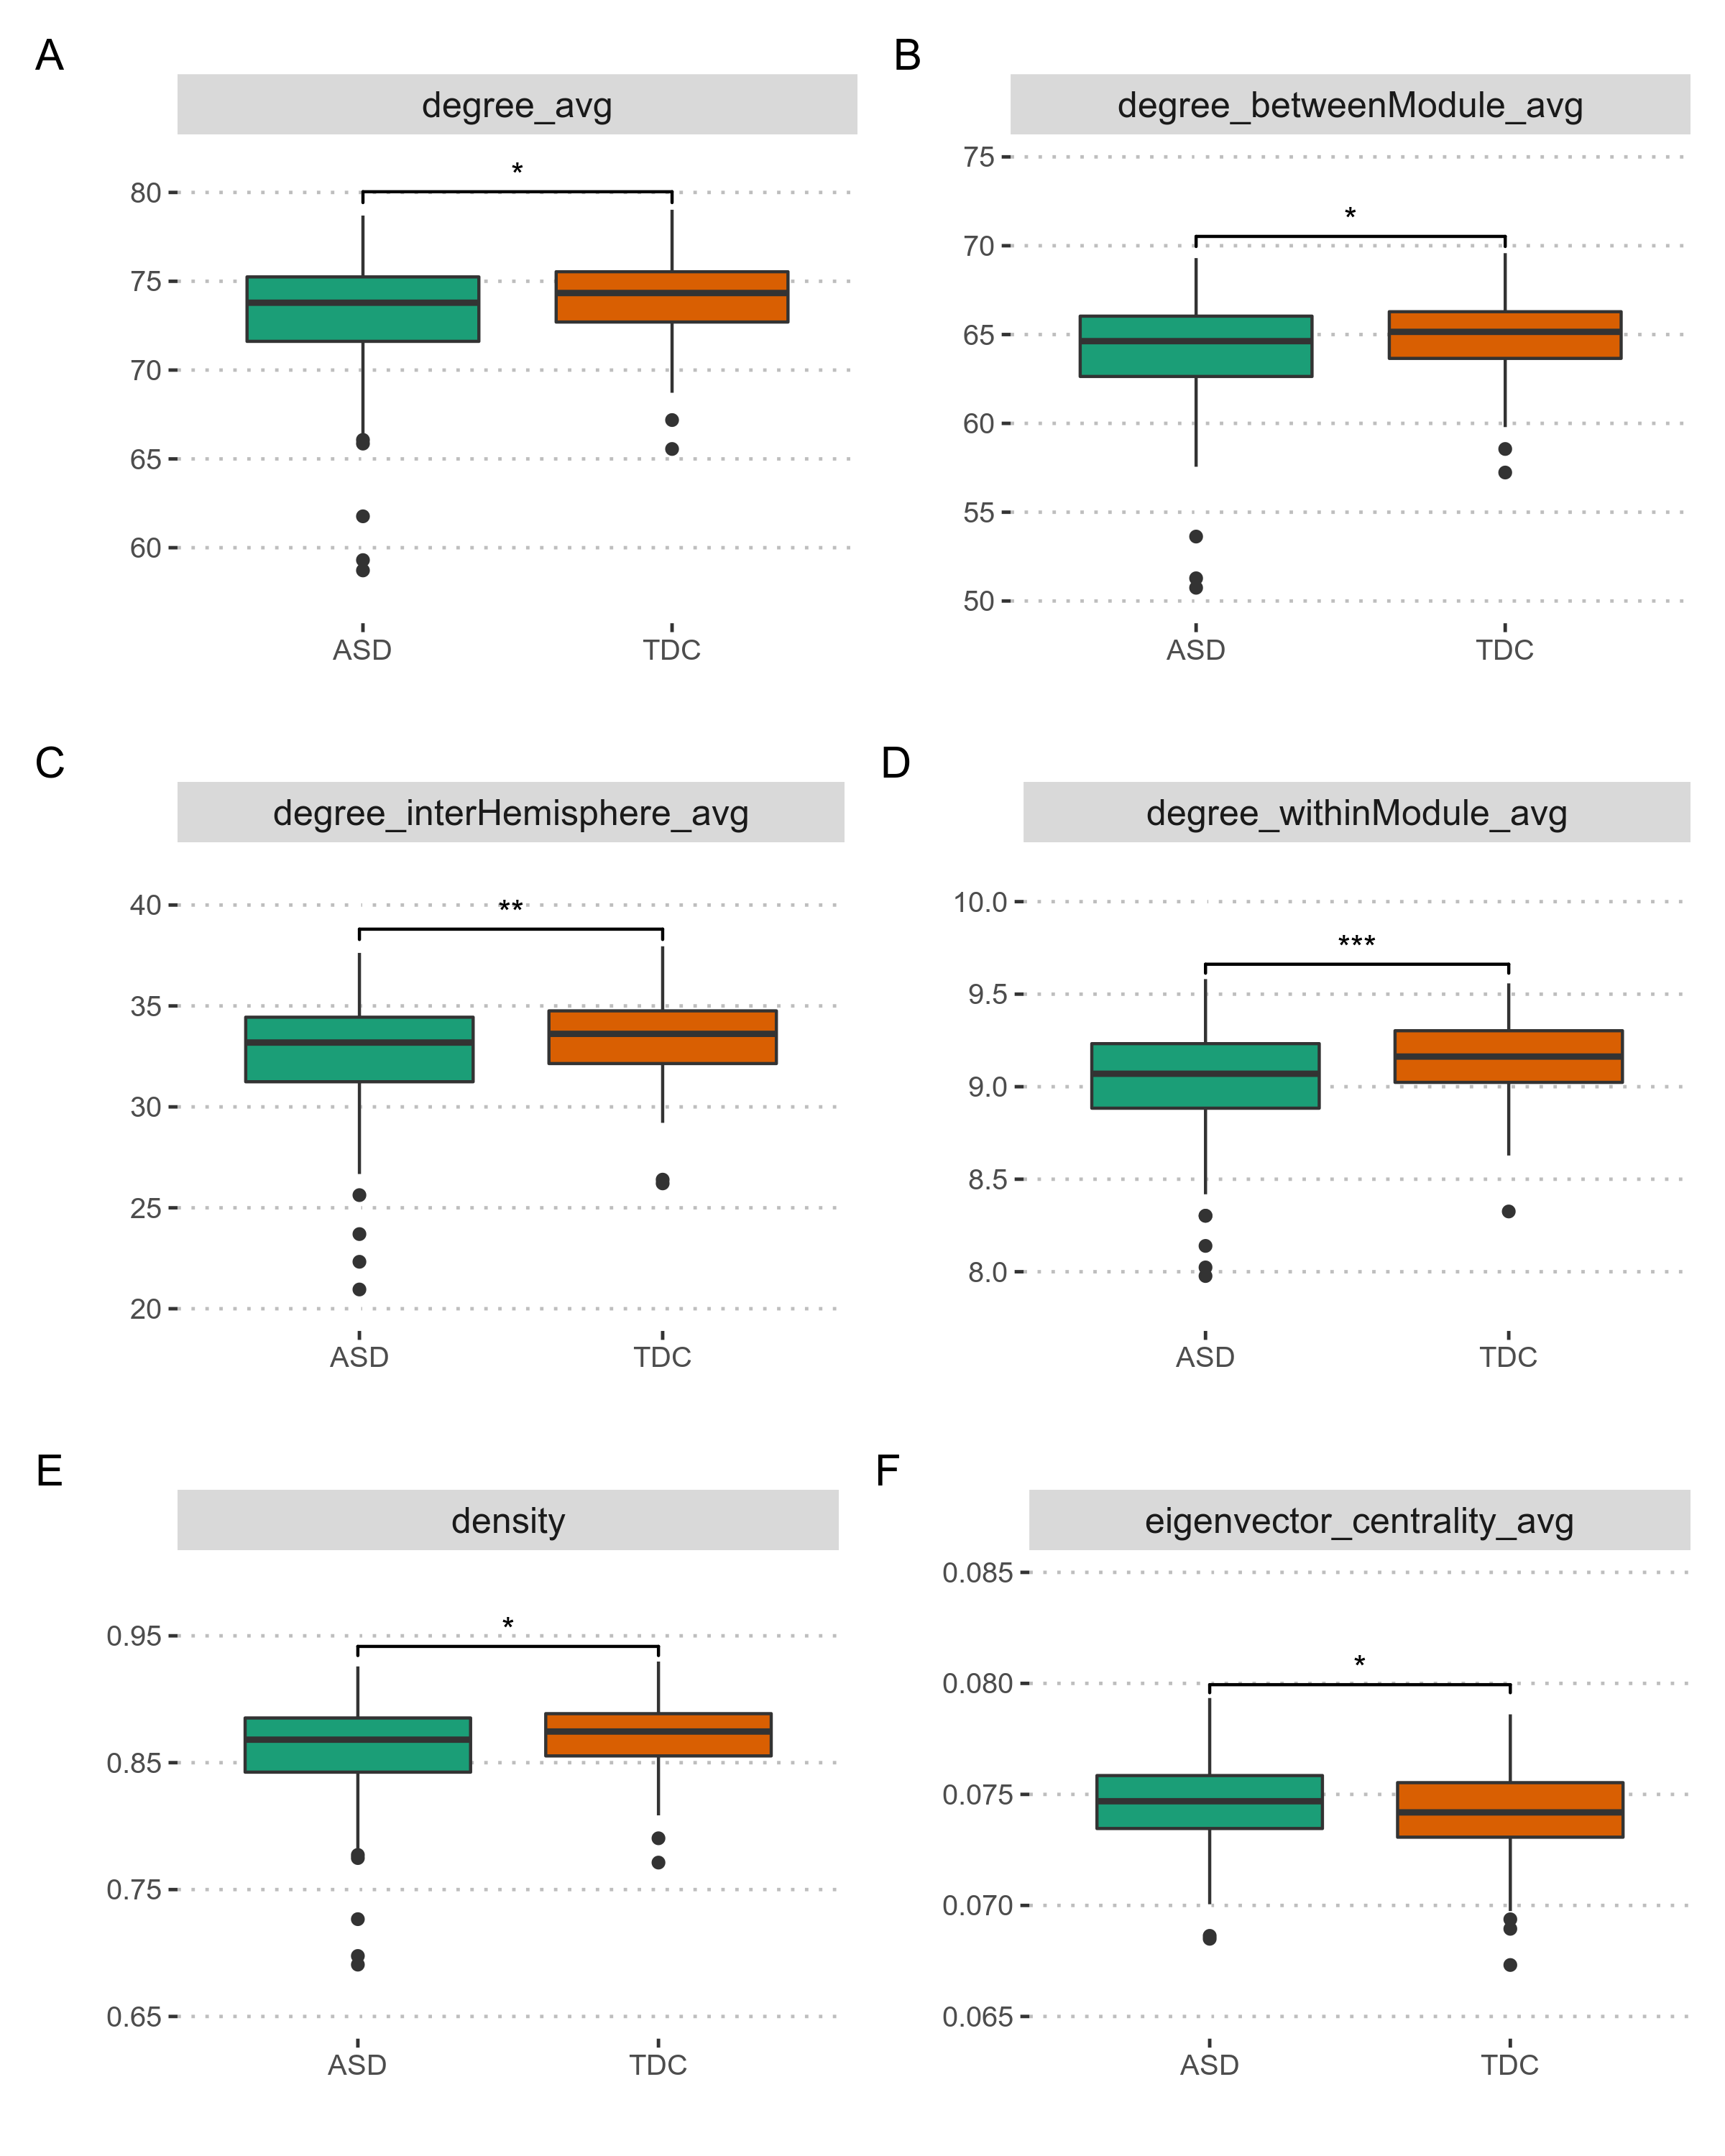
\includegraphics[width=\columnwidth]{../../AutismCNN/figures/group-diff_global-measures_boxplot.png}}
            \caption{
                Significant Group differences between ASD and TDC connectomes for six graph
                theory measures. The significance is indicated by the starts `*' above the
                braces in each sub-plot. (A) Average Degree (B) Average Degree Between Modules
                (C) Average Inter-Hemispheric Degree (D) Average Degree Within Modules
                (E) Network Density (F) Average Eigenvector Centrality
            }
            \label{group-diff-boxplots}
        \end{center}
        \vskip -0.2in
    \end{figure}

\subsection*{\textbf{Identification of Potential Biomarkers}}

    To perform feature selection, we created a set of candidate biomarkers based on the 
    results from the group difference analysis. Since no significant measures were 
    identified for the Schaefer connectomes, we chose to focus exclusively on the Desikan
    connectomes. The set of candidate biomarkers includes the following network-level 
    measures: `Average Degree', `Average Degree between and within Module', 
    `Average Interhemispheric Degree',  `Density', and `Average Eigenvector Centrality'.
    The corresponding node-level measures (except for `Density') were also included as 
    candidate biomarkers. In total, we included 436 candidate biomarkers for the Desikan 
    connectomes.

    The first set of potential biomarkers was identified using LASSO regression. The 
    training dataset was fit to the LASSO regression model and the optimal hyperparameters 
    were identified using `GridSearchCV' with 5-fold cross-validation. The optimal 
    regularization parameter was found to be 0.1 for Desikan connectomes. The network-level 
    and a node-level (Node 48) `Degree within Module' were the only features selected.

    The second set of potential biomarkers was identified using RFE with a SVC classifier. 
    The training dataset was fit to the LinearSVC and the optimal hyperparameters were 
    identified using `GridSearchCV' with 5-fold cross-validation. The optimal 
    regularization parameter was found to be 0.3. A total of 86 node-level features were 
    selected from the original 436; of these, 25 were Interhemispheric Degree (IHD) measures,
    23 were Degree between Module (DBM) measures, 16 were Degree within Module (DWM) 
    measures and 22 were Degree (D) measures.

\subsection*{\textbf{Diagnostic Accuracy of Potential Biomarkers}}

    The diagnostic accuracy of the two sets of potential biomarkers was evaluated using 
    the AUC-ROC curve metric. For the first set of potential biomarkers (selected by 
    LASSO regression), the AUC was 0.53. For the second set of potential biomarkers 
    (node-level only, selected by RFE with SVC), the AUC was 0.51. Additionally, we 
    calculated the AUC for `Average Degree within Module' since this was the only feature 
    present in both sets of biomarkers; the AUC was 0.59.

    \begin{figure}
        \vskip 0.2in
        \begin{center}
            \centerline{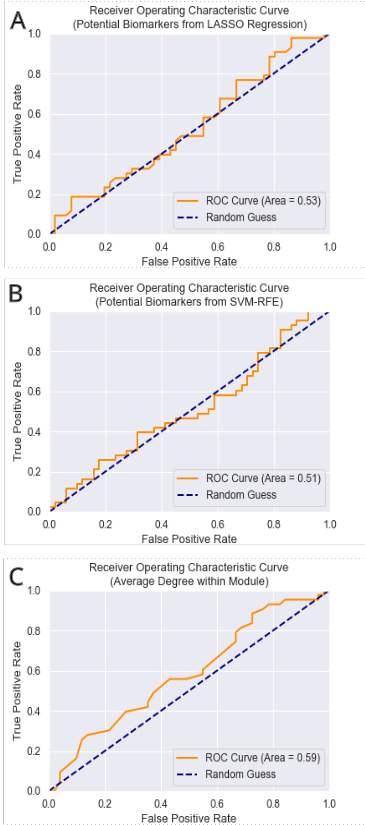
\includegraphics[width=2in]{../../AutismCNN/figures/roc.png}}
            \caption{
                Receiver Operating Characteristic (ROC) curves for different sets of features.
                (A) ROC curve for biomarkers identified by LASSO regression
                (B) ROC curve for biomarkers identified by RFE with a SVC classifier
                (C) ROC curve for the Average Degree within Module
            }
            \label{clinical-corrmap}
        \end{center}
        \vskip -0.2in
    \end{figure}

\subsection*{\textbf{Correlation with Clinical Outcomes}}

    The significant network-level graph theory measures were correlated with the ADOS-CSS, 
    SCQ and IQ scores. No significant correlations were observed between the SCQ or ADOS-CSS
    scores. The `Average Interhemispheric Degree' and `Average Degree within Module' were 
    found to exhibit significant, weak correlations with IQ scores among autistic children.
    Fig \ref{clinical-corrplots} shows scatter plots of the measures against IQ with a 
    line of best fit; the scatter plots are annotated with the correlation coefficients (R) 
    and p-values for each case.
    Both sets of potential biomarkers were combined and their correlations with the 
    clinical outcome scores (ADOS-CSS, SCQ, IQ) were calculated. The heatmap in Fig 
    \ref{clinical-corrmap} shows the correlations between the potential biomarkers and the 
    scores. The different types of node-level features are identified by the row colors in 
    the figure legend. 

    \begin{figure}
        \vskip 0.2in
        \begin{center}
            \centerline{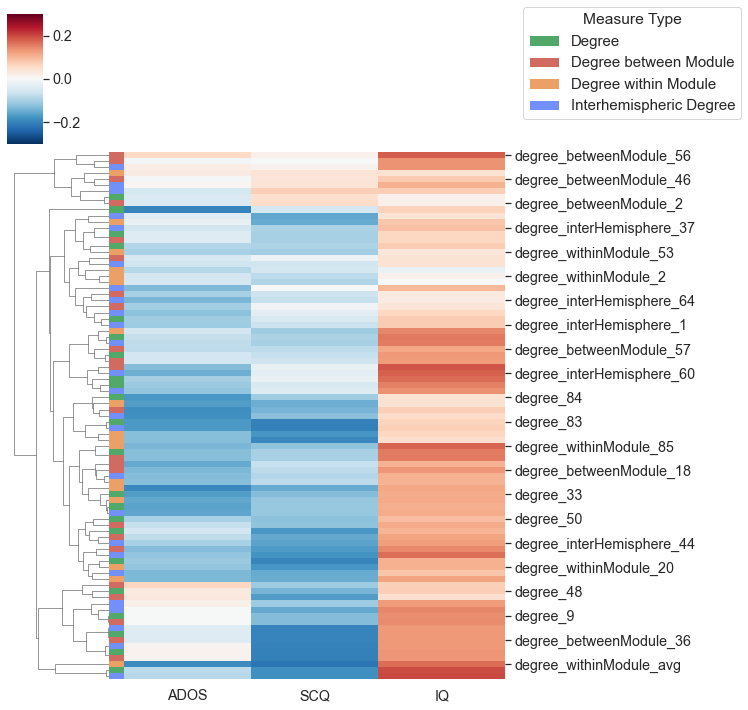
\includegraphics[width=\columnwidth]{../../AutismCNN/figures/clinical-corrmap.png}}
            \caption{
                Heatmap showing the correlation between the potential biomarkers and various 
                clinical outcomes (ADOS-CSS, SCQ, IQ). Rows are hierarchically clustered and 
                each type of feature is represented by a different color.
            }
            \label{clinical-corrmap}
        \end{center}
        \vskip -0.2in
    \end{figure}

    \begin{figure}
        \vskip 0.2in
        \begin{center}
            \centerline{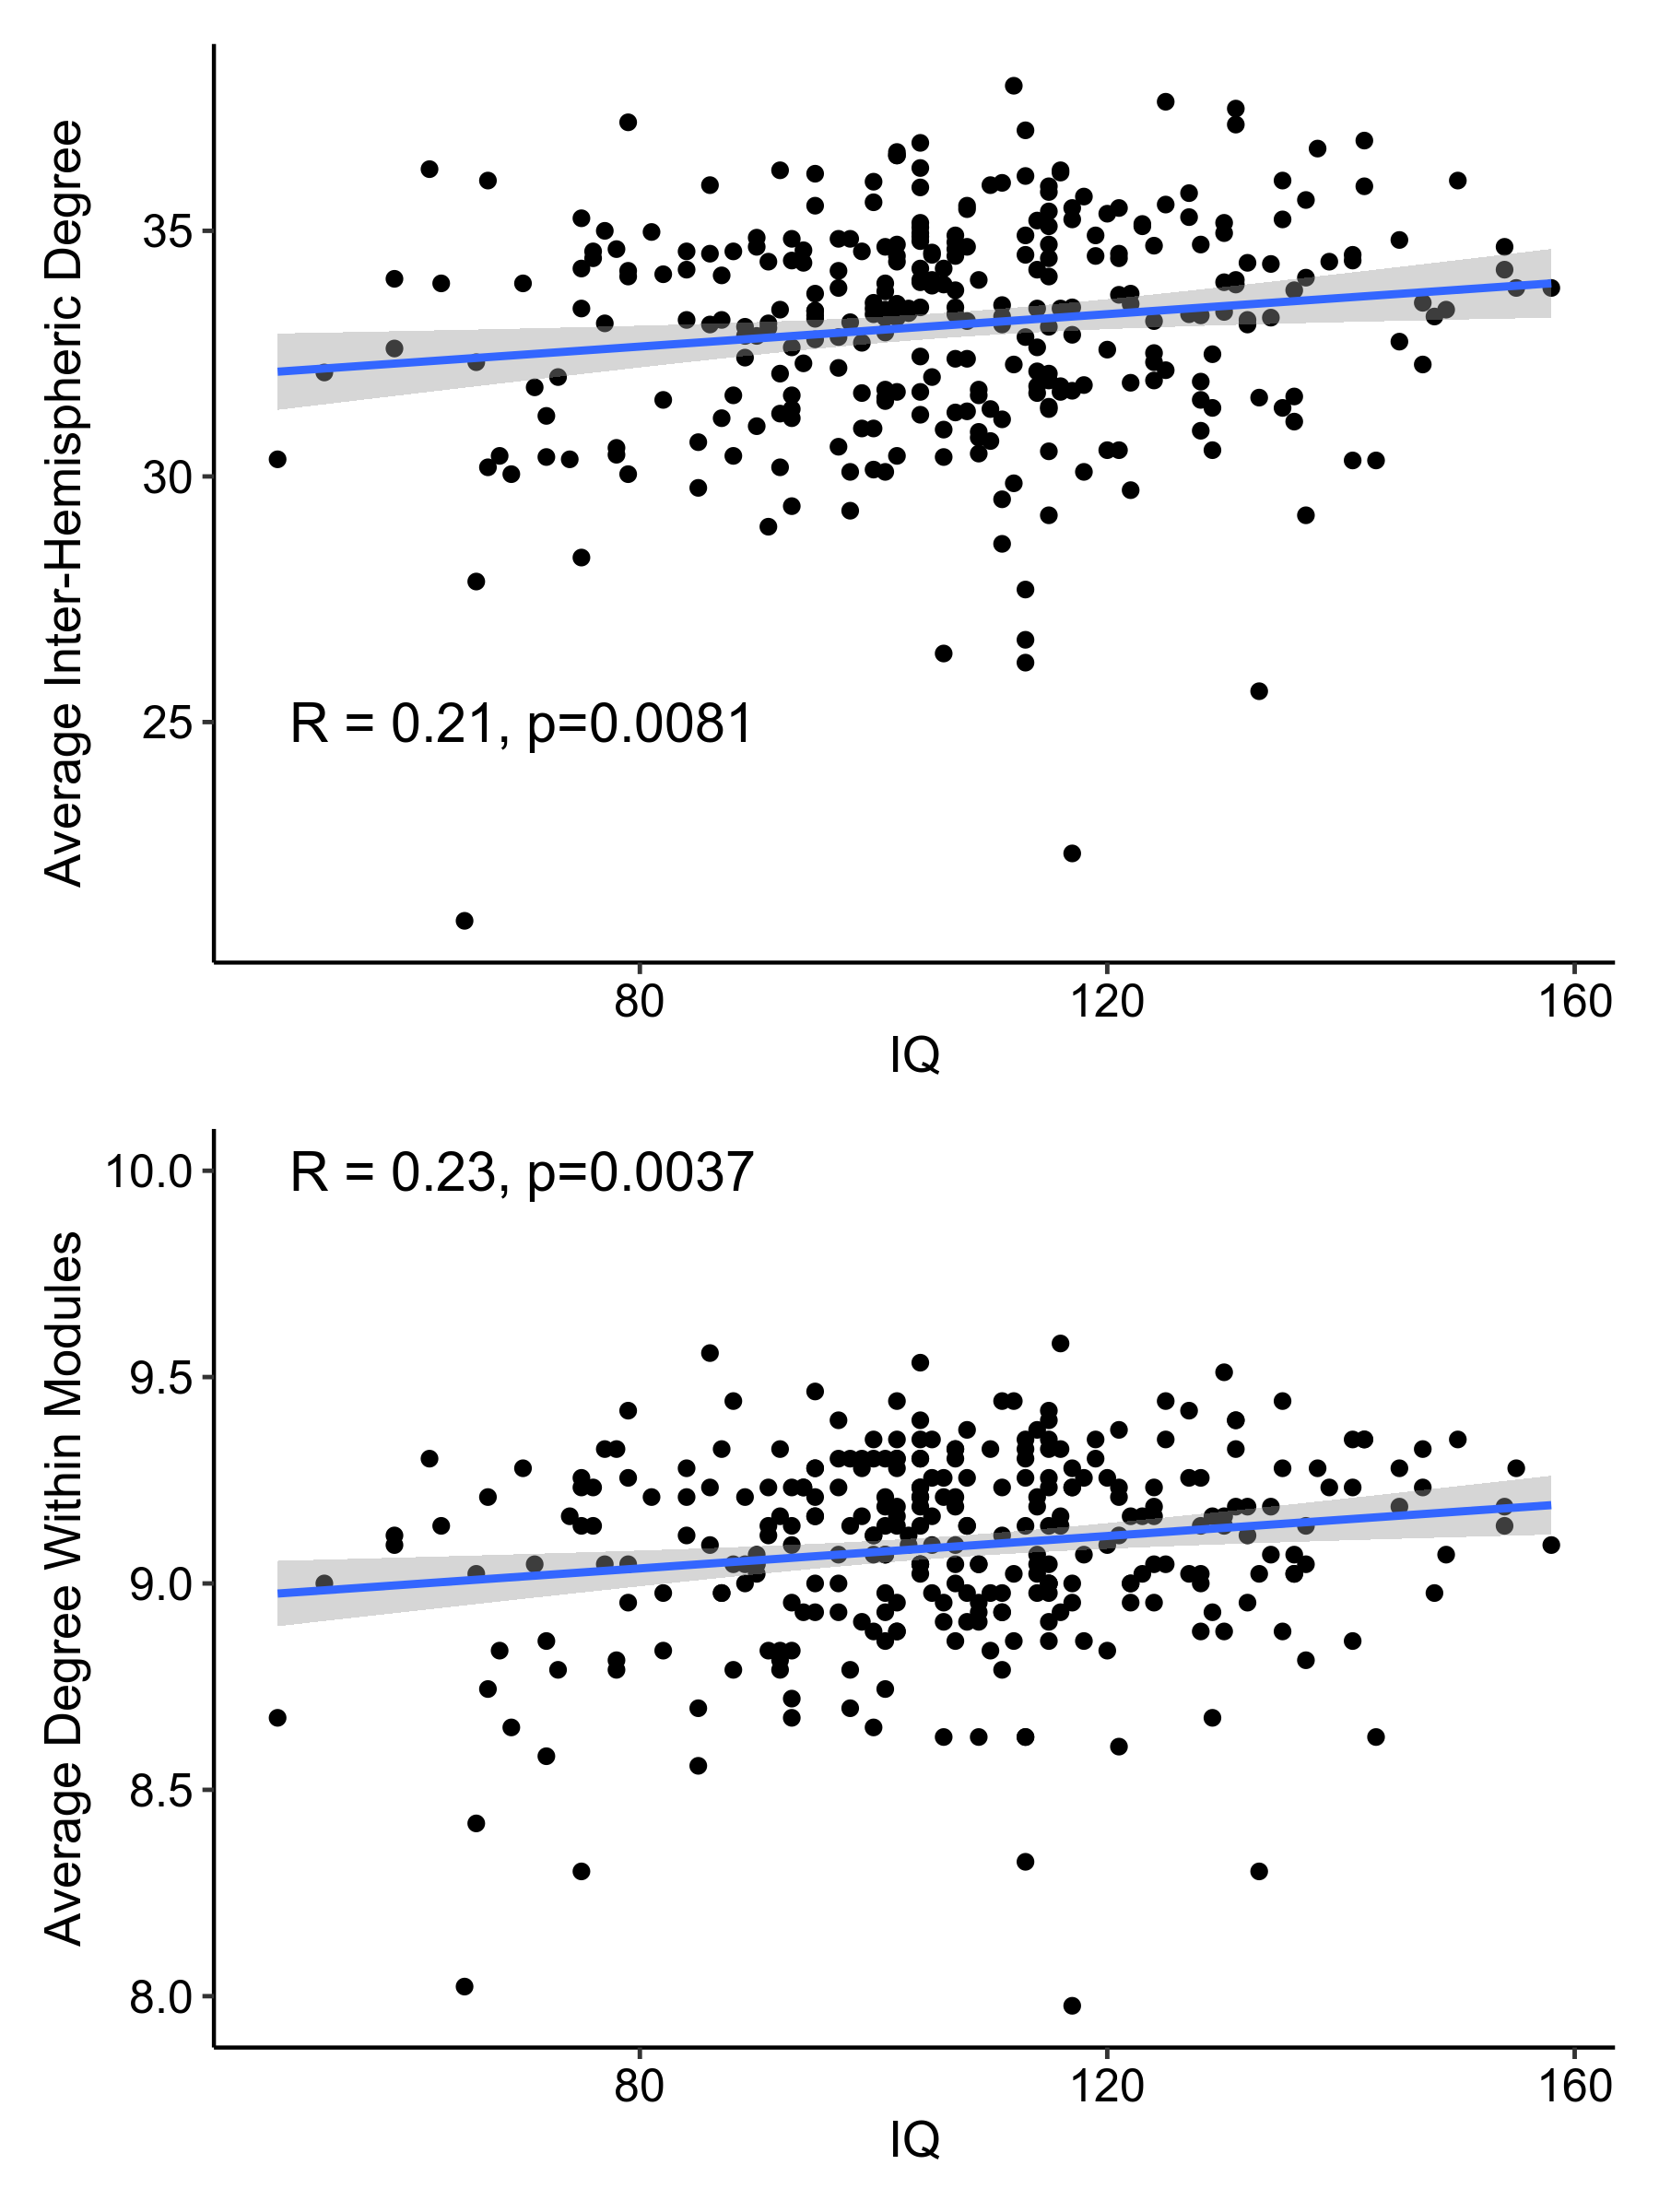
\includegraphics[width=3in]{../../AutismCNN/figures/corrplot_global-measures_boxplot.png}}
            \caption{
                Scatterplots with fitted linear regression lines for global graph theory 
                measures significantly correlated with IQ. (Top) Average Inter-Hemispheric 
                Degree  (Bottom) Average Degree Within Modules
            }
            \label{clinical-corrplots}
        \end{center}
        \vskip -0.2in
    \end{figure}

% ----------------------------------------------------------------------------------------

\section{Discussion}

We identified `Average Degree within Module' as the only significantly different measure
between ASD and TDC connectomes constructed with the Desikan atlas. This measure evaluates 
the magnitude of connectivity within brain subnetworks. A moderate effect size of -0.489 
was computed for this measure indicating that the ASD connectomes have fewer connections
within each brain subnetwork than the TDC connectomes do. This is of particular interest
since it suggests that the strength of neuronal connections within each subnetwork is 
decreased in Autistic brains which may suggest an increase in the overall global connectivity 
as well. To investigate this, we would suggest performing a subnetwork level anaysis of the 
connectomes to identify what subnetworks in particular are different between the two groups. 

The first set of potential biomarkers (selected by LASSO regression) exhibited an AUC of 
0.53 indicating that with only the 2 features selected, the model only performed slightly 
better that a random guess at predict whether a connectome came from a subject with ASD. 
This potentially suggests that a larger set of features would need to be identified to more 
accurately distinguish ASD from TDC.

The second set of potential biomarkers (node-level only, selected by RFE with SVC) \
exhibited an AUC of 0.51 indicating that this collection of 86 features was no better than 
a random guess at distinguishing ASD from TDC. This could indicate that further 
optimization is needed out the feature selection approach. Using a more robust 
cross-validation strategy could potentially improve the feature selection outcome. 
Additionally, the variations across the entire connectome could be difficult to capture 
with a simple linear kernel; further studies will explore the ability of non-linear 
kernels to better capture the variation in the dataset.

Finally, we also looked at the AUC ROC for the `Average Degree within Module' measure. This 
was the only significant measure identified and was present in one of the sets of potential 
biomarkers. Considering that a significant portion of node-level features in the second 
biomarker set were `Degree within Module' measures, we expected to see a higher diagnostic 
power for this measure. The AUC was 0.59 indicating a higher probability of true positives 
over false positives. This is promising because, as stated earlier, this measure describes 
whether a connectome is more similar to a modular network -- with high connectivity within 
subnetworks and low global connectivity -- or to a more well connected network. We plan to 
investigate this further by performing a subnetwork level analysis of the connectomes; this 
will involve extracting separate connectomes for subnetworks of interest and computing 
graph theory measures for those networks. This approach will allow us to better understand 
where the structural differences between autistic and typically developing brains are 
concentrated, and potentially reveal more accurate biomarkers for ASD diagnosis.
 

The other significant differences
in the Desikan connectomes indicate that nodes in the ASD
group have less degree on average, less connections across
brain modules, less connections within their own hemisphere,
less strongly weighted connections within their own hemisphere, and more strongly weighted connections which span
hemispheres.



% ----------------------------------------------------------------------------------------

\begin{thebibliography}{00}
    \bibitem{Abos.2017} {Abos, A., Baggio, H., Segura, B., Garcia-Diaz, A., Compta, Y., Marti, M., Valldeoriola, F., \& Junqué, C. (2017). Discriminating cognitive status in Parkinson's disease through functional connectomics and machine learning. Scientific reports, 7(1), 1–-13.}
    \bibitem{dAlBbis.2018} {d`Albis, M.A., Guevara, P., Guevara, M., Laidi, C., Boisgontier, J., Sarrazin, S., Duclap, D., Delorme, R., Bolognani, F., Czech, C., \& others (2018). Local structural connectivity is associated with social cognition in autism spectrum disorder. Brain, 141(12), 3472–-3481.}
    \bibitem{Craddock.2013} {Craddock, R., Jbabdi, S., Yan, C.G., Vogelstein, J., Castellanos, F., Di Martino, A., Kelly, C., Heberlein, K., Colcombe, S., \& Milham, M. (2013). Imaging human connectomes at the macroscale. Nature methods, 10(6), 524--539.}
    \bibitem{Hong.2019} {Hong, S.J., Wael, R., Bethlehem, R., Lariviere, S., Paquola, C., Valk, S., Milham, M., Di Martino, A., Margulies, D., Smallwood, J., \& others (2019). Atypical functional connectome hierarchy in autism. Nature communications, 10(1), 1--13.}
    \bibitem{Horien.2022} {Horien, C., Floris, D.L., Greene, A.S., Noble, S., Rolison, M., Tejavibulya, L., O'Connor, D., McPartland, J.C., Scheinost, D., Chawarska, K. and Lake, E.M., 2022. Functional connectome-based predictive modelling in autism. Biological Psychiatry.}
    \bibitem{Jubair.2020} {Jubair, S., Alkhateeb, A., Tabl, A. A., Rueda, L., \& Ngom, A. (2020). A novel approach to identify subtype-specific network biomarkers of breast cancer survivability. Network Modeling Analysis in Health Informatics and Bioinformatics, 9(1), 1-12.}
    \bibitem{Kawahara.2017} {Kawahara, J., Brown, C., Miller, S., Booth, B., Chau, V., Grunau, R., Zwicker, J., \& Hamarneh, G. (2017). BrainNetCNN: Convolutional neural networks for brain networks; towards predicting neurodevelopment. NeuroImage, 146, 1038--1049.}
    \bibitem{Lau.2019} {Lau, W., Leung, M.K., \& Lau, B. (2019). Resting-state abnormalities in autism spectrum disorders: a meta-analysis. Scientific reports, 9(1), 1--8.}
    \bibitem{Nunes.2019} {Nunes, A., Peatfield, N., Vakorin, V., \& Doesburg, S. (2019). Idiosyncratic organization of cortical networks in autism spectrum disorder. Neuroimage, 190, 182--190.}
    \bibitem{sklearn} {Pedregosa, F., Varoquaux, G., Gramfort, A., Michel, V., Thirion, B., Grisel, O., Blondel, M., Prettenhofer, P., Weiss, R. et. al. (2011). Scikit-learn: Machine Learning in Python. Journal of Machine Learning Research, 12(1), 2825-2830.}
    \bibitem{R-Core} {R Core Team (2022). R: A language and environment for statistical computing. R Foundation for Statistical Computing, Vienna, Austria. URL https://www.R-project.org/.}
    \bibitem{Roine.2015} {Roine, U., Roine, T., Salmi, J., Nieminen-von Wendt, T., Tani, P., ... \& Sams, M. (2015). Abnormal wiring of the connectome in adults with high-functioning autism spectrum disorder. Molecular Autism, 6(1), 1-11.}
    \bibitem{Rubinov.2010.BCT} {Rubinov, M., \& Sporns, O. (2010). Complex network measures of brain connectivity: uses and interpretations. Neuroimage, 52(3), 1059--1069.}
    \bibitem{Shen.2019} {Shen, L., Zhao, Y., Zhang, H., Feng, C., Gao, Y., Zhao, D., Xia, S., Hong, Q., Iqbal, J., Liu, X., \& others (2019). Advances in biomarker studies in autism spectrum disorders. Reviews on Biomarker Studies in Psychiatric and Neurodegenerative Disorders, 207–-233.}
    \bibitem{Vogt.2018} {Vogt, N. (2018). Machine learning in neuroscience. Nature Methods, 15(1), 33-33.}    
    \bibitem{ggplot2} {Wickham, H., ggplot2: Elegant Graphics for Data Analysis. Springer-Verlag New York, 2016.}
    \bibitem{Wang.2019} {Wang H, Lengerich BJ, Aragam B, Xing EP. Precision Lasso: accounting for correlations and linear dependencies in high-dimensional genomic data. Bioinformatics. 2019;35(7):1181-7.}
    \bibitem{Williams.2013} {Williams, D., Cherkassky, V., Mason, R., Keller, T., Minshew, N., \& Just, M. (2013). Brain function differences in language processing in children and adults with autism. Autism Research, 6(4), 288--302.}
    \bibitem{Zhang.2021} {Zhang, Y., Wei, X., Cao, C., Yu, F., Li, W., Zhao, G., ... \& Guo, X. (2021). Identifying discriminative features for diagnosis of Kashin-Beck disease among adolescents. BMC Musculoskeletal Disorders, 22(1), 1-10.}

\end{thebibliography}

\end{document}
